\subsection{Countermeasures}

\begin{frame}[t]
\begin{center}\Large Algebraic Security (1/3)\end{center}

\begin{columns}
    \setlength{\leftmargini}{0.25cm}
    \setlength{\leftmarginii}{0.5cm}
    \column{0.1\linewidth}{}
    \column{0.35\linewidth}{
        {\large Security Model:}
        \vspace{0.25cm}
        \begin{enumerate}
            \item<1-> \alert{random} bits allowed \\
                \begin{itemize}
                    \item as in classic masking
                    \item model~\alert{unpredictability}
                    \item in WB impl. as {\bf pseudorandom}
                \end{itemize}
            
            \item<2-> {\bf Goal:} \\
                  any $f \in span\{v_i\}$ is \alert{unpredictable}
                  
            \item<3-> {\bf isolated} from obfuscation problems
        \end{enumerate}
    }
    \column{0.5\linewidth}{
        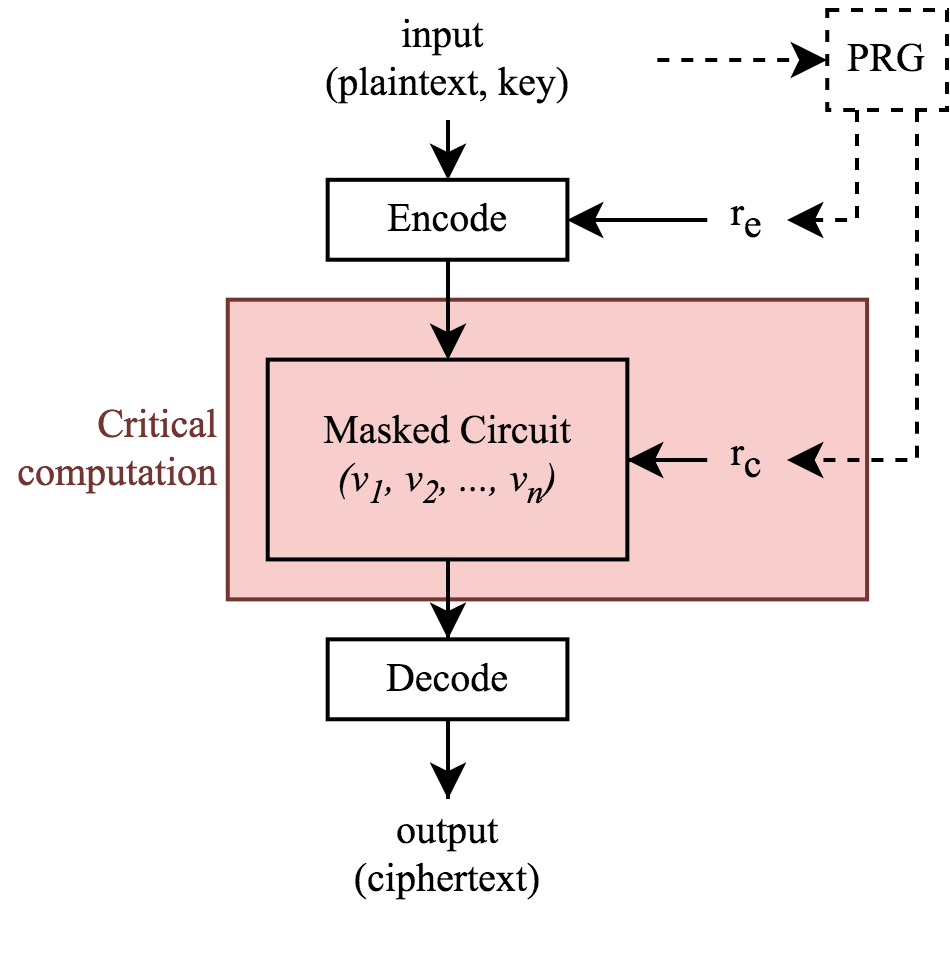
\includegraphics[height=7cm]{MaskedCircuitWB.png}
    }
\end{columns}
\end{frame}

\newcommand\bias{\varepsilon}
\newcommand\adv{\mathcal{A}}
\newcommand\Advan{\mathsf{Adv}}

\begin{frame}[t]
\begin{center}\Large Algebraic Security (2/3)\end{center}

\begin{columns}
    \setlength{\leftmargini}{0.25cm}
    \setlength{\leftmarginii}{0.5cm}
    \column{0.1\linewidth}{}
    \column{0.35\linewidth}{
        {\large Adversary:}
        \vspace{0.25cm}
        \begin{enumerate}
            \item<1-> chooses plaintext/key pairs
            
            \item<2-> chooses $f \in span\{v_i\}$
            \item<3-> tries to {\bf predict} values of this function \\ 
                  (i.e. before random bits are sampled)
            
            %\item<4-> succeeds,\\
            %      if \alert{only} $f$ matches
        \end{enumerate}
    }
    \column{0.5\linewidth}{
        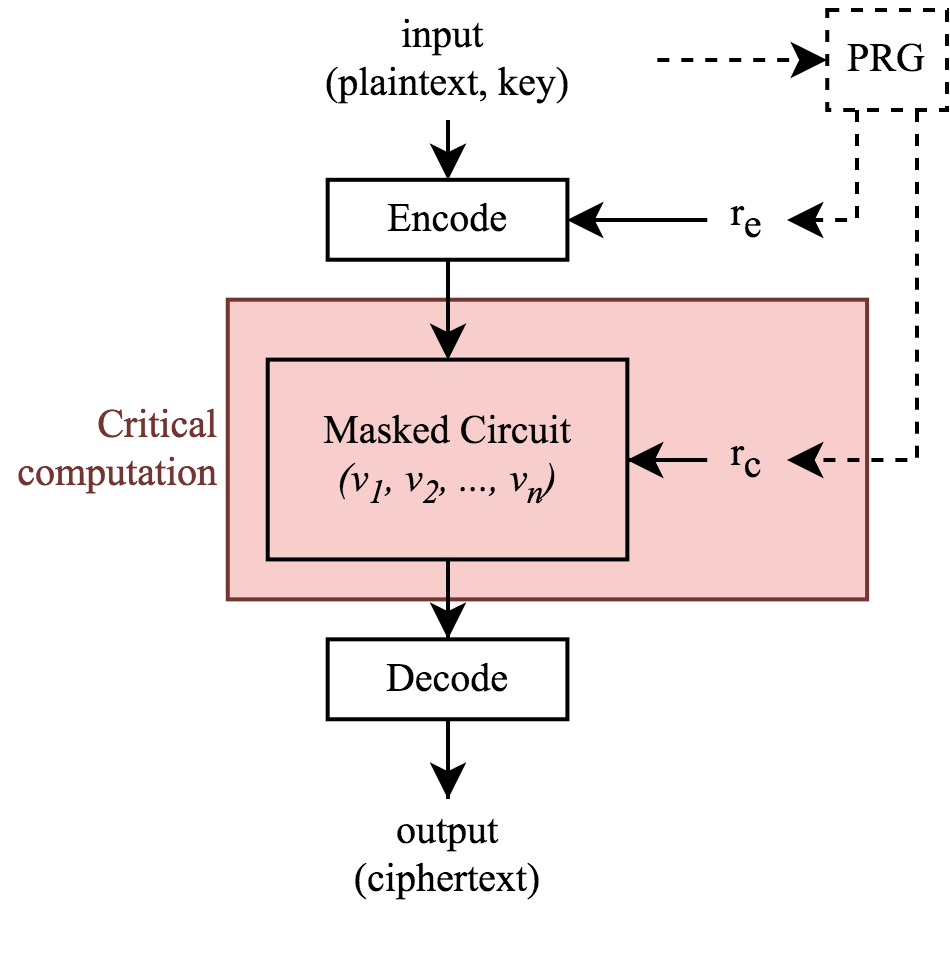
\includegraphics[height=7cm]{MaskedCircuitWB.png}
    }
\end{columns}
\end{frame}


\begin{frame}
\begin{center}\Large Algebraic Security (3/3)\end{center}

\CenterBlock{10cm}{
\begin{block}{Proposition}

Let ${\color{blue}F} = \{f(x,\cdot,\cdot) ~\mid~ f(x,r_e,r_c) \in span\{v_i\},~ x \in \mathbb{F}_2^N\}.$

Let ${\color{red}e} = -\log_2{\big(1/2 + \max_{f \in {\color{blue}F}}{bias(f)}\big)}$.

Then for any adversary $\adv$ choosing $Q$ inputs
$$
    \Advan[\adv] \le min(2^{Q-|r_c|}, 2^{-{\color{red}e}Q}).
$$
\end{block}
}

\pause 

\CenterBlock{10cm}{
\begin{block}{Corollary}
Let ${\color{green!40!black}k}$ be a positive integer. Then for any adversary $\adv$
$$
    \Advan[\adv] \le 2^{-{\color{green!40!black}k}} \text{~if~}
    e > 0 \text{~and~} |r_c| \ge k\cdot(1+\frac{1}{{\color{red}e}}).
$$
\end{block}
}

\pause 

\center{\bf Information-theoretic security!}
\end{frame}

\begin{frame}[t]
    \Title{Minimalist Quadratic Masking Scheme}
    \begin{columns}
    \setlength{\leftmargini}{0.5cm}
    \column{0.1\linewidth}{}
    \column{0.3\textwidth}{
        \only<1>{
            {\Large Masking scheme}
            \vspace{0.25cm}
            \begin{itemize}
                \item \alert{quadratic} decoder:\\
                      $(a,b,c) \mapsto ab\oplus c$
                \item set of {\bf gadgets} \\
                \item provably secure {\bf composition}
            \end{itemize}
        }
        \only<2->{
            {\Large Security}
            \vspace{0.25cm}
            \begin{enumerate}
                \item algorithm to verify \\
                      that bias $\ne 1/2$
                \item max. degree on $r$: 4
            \end{enumerate}
            \onslide<3->{
            
            \vspace{0.3cm}
            
            ~~~~$\Rightarrow$ bias $\le 7/16$
            
            \vspace{0.3cm}
            
            ~~~~for 80-bit security \\
            ~~~~we need $|r_c| \ge 940$
            }
        }
    }
    \column{0.5\textwidth}{
        \tiny
        \begin{algorithmic}
            % \Function{Encode}{$x,r_a,r_b$}
            %     \State \Return{$(r_a,r_b,r_ar_b \oplus x)$}
            % \EndFunction
            % \Statex
            % \Function{Decode}{$a,b,c$}
            %     \State \Return{$ab\oplus c$}
            % \EndFunction
            % \Statex
            \Function{EvalXOR}{$(a,b,c),(d,e,f),(r_a,r_b,r_c),(r_d,r_e,r_f)$}
                \State $(a,b,c) \gets \textsc{Refresh}((a,b,c),(r_a,r_b,r_c))$
                \State $(d,e,f) \gets \textsc{Refresh}((d,e,f),(r_d,r_e,r_f))$
                \State $x \gets a \oplus d$
                \State $y \gets b \oplus e$
                \State $z \gets c \oplus f \oplus ae \oplus bd$
                \State \Return{$(x,y,z)$}
            \EndFunction
            \Statex
            \Function{EvalAND}{$(a,b,c),(d,e,f),(r_a,r_b,r_c),(r_d,r_e,r_f)$}
                \State $(a,b,c) \gets \textsc{Refresh}((a,b,c),(r_a,r_b,r_c))$
                \State $(d,e,f) \gets \textsc{Refresh}((d,e,f),(r_d,r_e,r_f))$
                \State $m_a \gets bf \oplus r_c e$
                \State $m_d \gets ce \oplus r_f b$
                \State $x \gets ae \oplus r_f$
                \State $y \gets bd \oplus r_c$
                \State $z \gets am_a \oplus dm_d \oplus r_c r_f \oplus cf$
                \State \Return{$(x,y,z)$}
            \EndFunction
            \Statex
            \Function{Refresh}{$(a,b,c),(r_a,r_b,r_c)$}
                \State $m_a \gets r_a \cdot (b \oplus r_c)$
                \State $m_b \gets r_b \cdot (a \oplus r_c)$
                \State $r_c \gets
                    m_a \oplus m_b \oplus
                    (r_a \oplus r_c) (r_b \oplus r_c) \oplus
                    r_c$
                \State $a \gets a \oplus r_a$
                \State $b \gets b \oplus r_b$
                \State $c \gets c \oplus r_c$
                \State \Return{$(a,b,c)$}
            \EndFunction
        \end{algorithmic}
    }
    \end{columns}
\end{frame}

\begin{frame}
\Title{Proof-of-concept masked AES-128}

\CenterBlock{10cm}{
\vspace{0.5cm}
\begin{enumerate}
    \item MQMS + 1-st order Boolean masking
    \item 31,783 $\to$ 2,588,743 gates expansion (x81)
    \item 16 Mb code / 1 Kb RAM / 0.05s per block on a laptop
    \item (unoptimized)
\end{enumerate}
}

\vspace{0.5cm}

\center{\Large
    \href{https://github.com/cryptolu/whitebox}{github.com/cryptolu/whitebox}
}
    
\end{frame}